\chapter{拡散性の評価}

\section{評価基準}
1章でも述べた通り、ホール空間は吸音面が1階客席面に偏在する非完全拡散音場である。
ここで、座席面遠方音場は大きな吸音力を持つ座席面から離れることにより、音場がより拡散した状態になるという推測のもと、拡散性の観点から評価を行う。
\\ さて、関連した用語として従来より残響理論の仮定として用いられる「完全拡散音場」がある。これは、次の2条件を満たす音場のことである。
\\(i)音響エネルギが室内全体に均一に分布していること。
\\(i\hspace{-.05em}i)どの点においても音の進行方向があらゆる方向に一様であること。
\\ 物理的な拡散性を言及するにあたり上記2条件を拡散性評価の軸とする。すなわち、(i)で音響エネルギ分布の一様性を、(ii)で反射音方向分布の一様性を評価する。各評価項目を\figref{kakusan}に示す。
以上を基に、本研究では物理的評価に立脚した音場の拡散性評価を行う。
\vspace{0.8cm}
\begin{figure}[htbp]
    \centering
    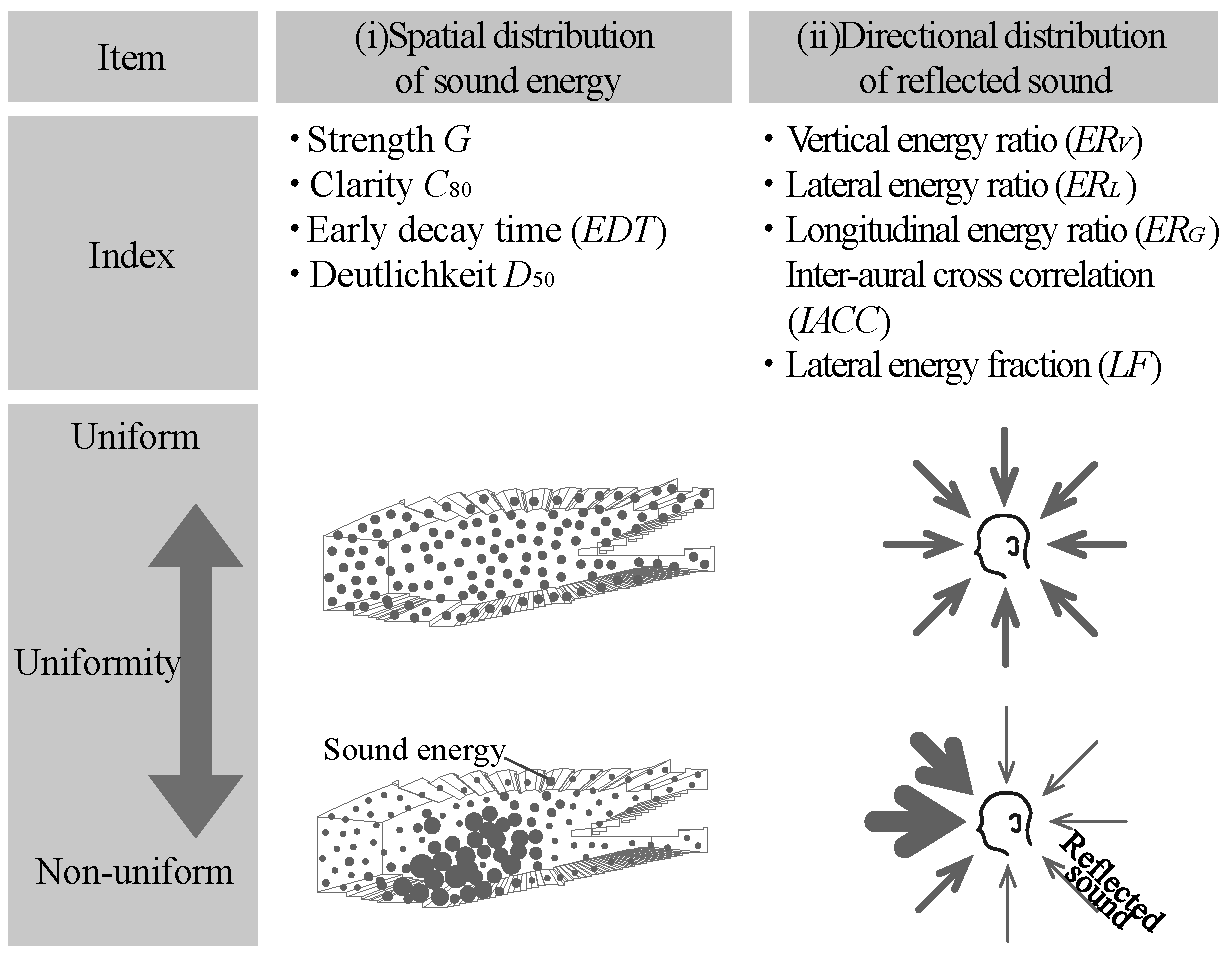
\includegraphics[keepaspectratio,scale=0.6]{01_att/kakusan.pdf}
    \caption{\hspace{1mm}Evaluation of diffusivity of sound field}
    \label{fig:kakusan}
\end{figure}

\pagebreak
\section{評価手法}
オーディトリウムで得られた測定値を定量化するため、統計的手法を用いる。
\subsection{平均値}
ホールの全観測点から算出した平均値は単一の値で音響特性を言い表す便利な値である。
しかしながら、残響時間を除く多くの音響物理量(明瞭性や音量感など)の平均値は観測位置により大きく異なる値から算出される可能性があり$^{\text{\cite{barron2005using}}}$、これは音響性能が全く異なる2つのホールが同じ平均値を取りうることを意味する。Barronは好意的な主観的印象を得るホールと聴衆にあまり受け入れられないホールの2つの例を示し、両ホールにおける主観的印象の平均値はほんのわずかな違いであったと述べている$^{\text{\cite{barron2002value}}}$。すなわち、主観的印象が全く異なるにも関わらず、ホールの平均値が非常に近い値をとる場合がある。
\\ これらのことから、平均値を用いた評価をする際はそのホール全体の分布をみる必要がある。
\subsection{標準偏差}
ISO 3382-1$^{\text{\cite{iso3382}}}$では空間における音響物理量の一様性をみる方法として標準偏差が使われている。
平均値が同じで標準偏差が異なる2つのホールを考えるとき、標準偏差が小さいホールがより音響エネルギが一様である。
ホールによっては中音域での$C_{80}$が正規分布をとらないという実測調査による報告$^{\text{\cite{akama2010distribution}}}$もあることから、標準偏差の利用にあたっては分布が正規分布となるかを念頭に置く必要がある。
\\ これらより、本研究では音響エネルギ分布の一様性を定量的に評価するため、標準偏差を用いる。

\subsection{一元配置分散分析}
1つの因子からなるデータを分析する方法であり、因子に含まれる水準間の平均値の差を見ることができる。本研究において、因子は音響物理指標、水準は観測高さが相当する。すなわち、解析モデル内の観測高さ$H$=1.2, 2.0, …14.0における音響物理指標値から一元配置分散分析を用いて、
$H$=1.2, 2.0, …14.0の音響物理指標値の平均点に差があるかどうかを検定する$^{\text{\cite{kanno}{\cite{池田1}{\cite{池田2}{\cite{池田3}}}}}}$。
\\ また、扱うデータが全て異なる被験者から得たデータ(被験者間のデータ)の場合は対応のないデータとして、同じ被験者から異なる水準で得たデータ(被験者内のデータ)の場合は対応のあるデータとして分析に用いる必要がある。本研究で用いるデータは、観測高さ(=水準)と共に観測点(x,y,$H_z$)(=被験者)のz値が変化することから対応のあるデータとして扱う。また、分析によって有意差が確認できた指標についてはどの観測高さ間に差があるのかを明らかにするため、Holm法による多重比較を行う。

\subsection{室内音響物理指標の弁別限}
観測高さ間に有意な差があったとき、その差は人間が知覚できるほどの変化量であるかどうかをJND ( just noticeable difference : 感覚上ちょうど感知できる物理刺激の最小変化量 ) を用いて判断する。
ISO3382-1$^{\text{\cite{iso3382}}}$に整理されている室内音響物理指標の弁別限(JND)を\tabref{jnd}に示す。
\begin{table}[htbp]
\centering
\caption{\hspace{1mm}JND of each acoustic parameters}
\label{tab:jnd}
\begin{tabular}{lccc}
\Hline
\multicolumn{1}{c}{Subjective listener aspect} & Acoustic quantity & \begin{tabular}[c]{@{}c@{}}Single number\\ freq. ave.$^*${[}Hz{]}\end{tabular} & \begin{tabular}[c]{@{}c@{}}Just noticeable difference\\ (JND)\end{tabular} \\ \hline
Subjective level of sound & $G${[}dB{]} & 500 to 1000 & 1[dB] \\
Perceived reverberance & $EDT${[}s{]} & 500 to 1000 & Rel.5[\%] \\
Perceived clarity of sound & $C_{80}${[}dB{]} & 500 to 1000 & 1[dB] \\
" & $D_{50}${[}\%{]} & 500 to 1000 & 5{[}\%{]} \\
Apparent source width (ASW) & $LF${[}\%{]} & 500 to 1000 & 5{[}\%{]} \\
\Hline
\multicolumn{4}{l}{$^{*}$ : The single number frequency averaging denotes the arithmetical average for the octave bands.}
\end{tabular}
\end{table}

\pagebreak
\subsection{室内音圧レベル分布に関する理論値}
従来の室内音響理論においては、拡散音の音圧レベルは距離によらず一定になる。
しかし、コンサートホールの実測調査では、これに当てはまらない結果を示すものがあった。
そこでBarronは拡散音が距離によって減衰するというrevised theory$^{\text{\cite{barron1988energy}}}$を提案している。
本研究では解析で得られた値をこれと共に示す。
\\ Barron's revised theoryではインパルス応答を直接音($d$)、初期反射音領域($e_r$ : t \textless 80 ms)、後期反射音領域($l$ : t \textgreater 80 ms)と時間軸上で分けて扱っている。ここで、$r$は音源-観測点間距離[m]、$T$は残響時間[s]、$V$は室容積[m$^3$]を表す。
\begin{table}[htbp]
    \begin{equation}
        \label{eq:d}
        d=\frac{100}{r^2}
    \end{equation}
    \begin{equation}
        e_r=\frac{31200T}{V}e^{\frac{-0.04r}{T}}(1-e^{\frac{-1.11}{T}})
    \end{equation}
    \begin{equation}
        l=\frac{31200T}{V}e^{\frac{-0.04r}{T}}e^{\frac{-1.11}{T}}
    \end{equation}
\end{table}
\\ $d$、$e_r$、$l$を用いて室内音響物理指標$G$や$G_{early}$,$G_{late}$,$C_{80}$の理論値を算出し、これと解析値との比較検討を行う。
\begin{table}[htbp]
    \begin{equation}
        G=10\log_{10}(d+e_r+l)\hspace{2mm}\dB
    \end{equation}
    \begin{equation}
        G_{early}=10\log_{10}(d+e_r)\hspace{2mm}\dB
    \end{equation}
    \begin{equation}
        G_{late}=10\log_{10}(l)\hspace{2mm}\dB
    \end{equation}
    \begin{equation}
        C_{80}=10\log_{10}(\frac{d+e_r}{l})\hspace{2mm}\dB
    \end{equation}

%        \begin{equation}
%        G_{early}=10\log_{10}(d+e_r)\hspace{2mm}\dB
%    \begin{equation}
%        VG_{early}=LG_{early}=GG_{early}=10\log_{10}\frac{d+e_r}{3}\hspace{2mm}\dB
%   \end{equation}
\end{table}